\section{Surat Pernyataan Penggunaan AI}

Dengan ini, kami: \\[.5em]
    \begin{tabular}{ll}
        \textbf{Nama/NIM} & : Zulfaqqar Nayaka Athadiansyah / 13523094 \\
        \textbf{Fakultas/Sekolah} & : Sekolah Teknik Elektro dan Informatika \\
        \textbf{Kode Mata Kuliah} & : IF3270 \\
        \textbf{Nama Mata Kuliah} & : Pembelajaran Mesin \\
        \textbf{Judul Tugas/Proposal} & : Tugas Besar 2: Convolutional Neural Network dan Recurrent Neural Network \\
    \end{tabular}

\vspace{0.5cm}

\noindent menyatakan bahwa kami \textbf{menggunakan} AI dalam pengerjaan maupun penyusunan luaran tugas pada mata kuliah yang tertulis di atas. \\

\noindent Jika \textbf{Ya}, maka alat AI/kecerdasan buatan yang digunakan adalah:

\vspace{0.1cm}

\begin{table}[H]
    \centering
    \small
    \renewcommand{\arraystretch}{1.5}
    \begin{tabular}{|L{7cm}|c|L{4cm}|}
        \hline
        \textbf{Lingkup Pekerjaan} & \textbf{Digunakan?} & \textbf{Tingkat Penggunaan} \\ \hline
        \textbf{Pemeriksaan Ejaan:} Grammarly, Paperpal, DeepL, Quillbot, ChatGPT, Gemini, dsb. & Tidak & \\ \hline
        \textbf{Pembuatan Teks:} ChatGPT, Gemini, Copilot, Jasper, Jenni AI, dsb. & Tidak & \\ \hline
        \textbf{Bantuan Diskusi/Konten:} Perplexity, ChatGPT, Zoom-Companion, dsb. & Ya & Untuk brainstorming awal, pembagian tugas, dan strategi implementasi \\ \hline
        \textbf{Grafik/Multimedia:} DALL-E, Midjourney, Stable Diffusion, Canva AI, dsb. & Tidak & \\ \hline
        \textbf{Lainnya:} & Tidak & \\ \hline
    \end{tabular}
\end{table}

\vspace{0.5cm}

\noindent Kami juga menyatakan bahwa setiap penggunaan AI/kecerdasan buatan yang dilakukan pada mata kuliah tersebut telah dinyatakan di dalam surat ini secara jujur dan transparan.

\vspace{1cm}

\begin{flushright}
    \begin{tabular}{c}
        Bandung, 15 Mei 2026 \\
        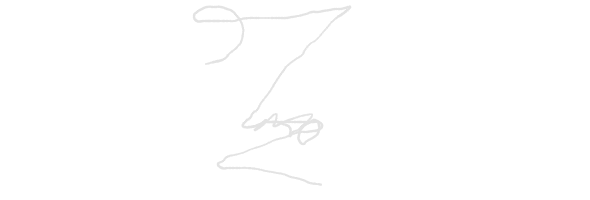
\includegraphics[scale=0.4]{assets/ttd.png}\\
        \textbf{\underline{\hspace{5cm}}} \\
        Zulfaqqar Nayaka Athadiansyah
    \end{tabular}
\end{flushright}

\vfill